\documentclass[a4paper,11pt,dvipdfmx]{jsarticle}


% 数式
\usepackage{amsmath,amsfonts}
\usepackage{bm}

% 画像
\usepackage[dvipdfmx]{graphicx}
\usepackage{framed}

% 図形
\usepackage{tikz}
\usetikzlibrary{shapes.geometric}
\usetikzlibrary {shapes.misc}

% ソースコード
\usepackage{listings,jlisting,color}
\lstset{
basicstyle={\ttfamily},
identifierstyle={\small},
commentstyle={\smallitshape},
keywordstyle={\small\bfseries},
ndkeywordstyle={\small},
stringstyle={\small\ttfamily},
frame={tb},
breaklines=true,
columns=[l]{fullflexible},
numbers=left,
xrightmargin=0zw,
xleftmargin=3zw,
numberstyle={\scriptsize},
stepnumber=1,
numbersep=1zw,
lineskip=-0.5ex
}
\renewcommand{\lstlistingname}{ソースコード}


\begin{document}
\definecolor{shadecolor}{gray}{0.70}

\title{画像処理 課題2 フィルタリング}
\author{21T2166D 渡辺大樹}
\date{\today}
\maketitle

\section{課題の目的・意図}
本課題では、ノイズを付加した画像をメジアンフィルタとバイラテラルフィルタの二種類で平滑化し、
それぞれのフィルタの特性や処理の得意なノイズを考察、特定することを目的とし行う。

\section{処理内容}
まず目的の画像、今回は図\ref{Morita}に示す画像にガウシアンノイズとソルト\&ペッパーノイズを付加する。
\begin{figure}[h]
\centering
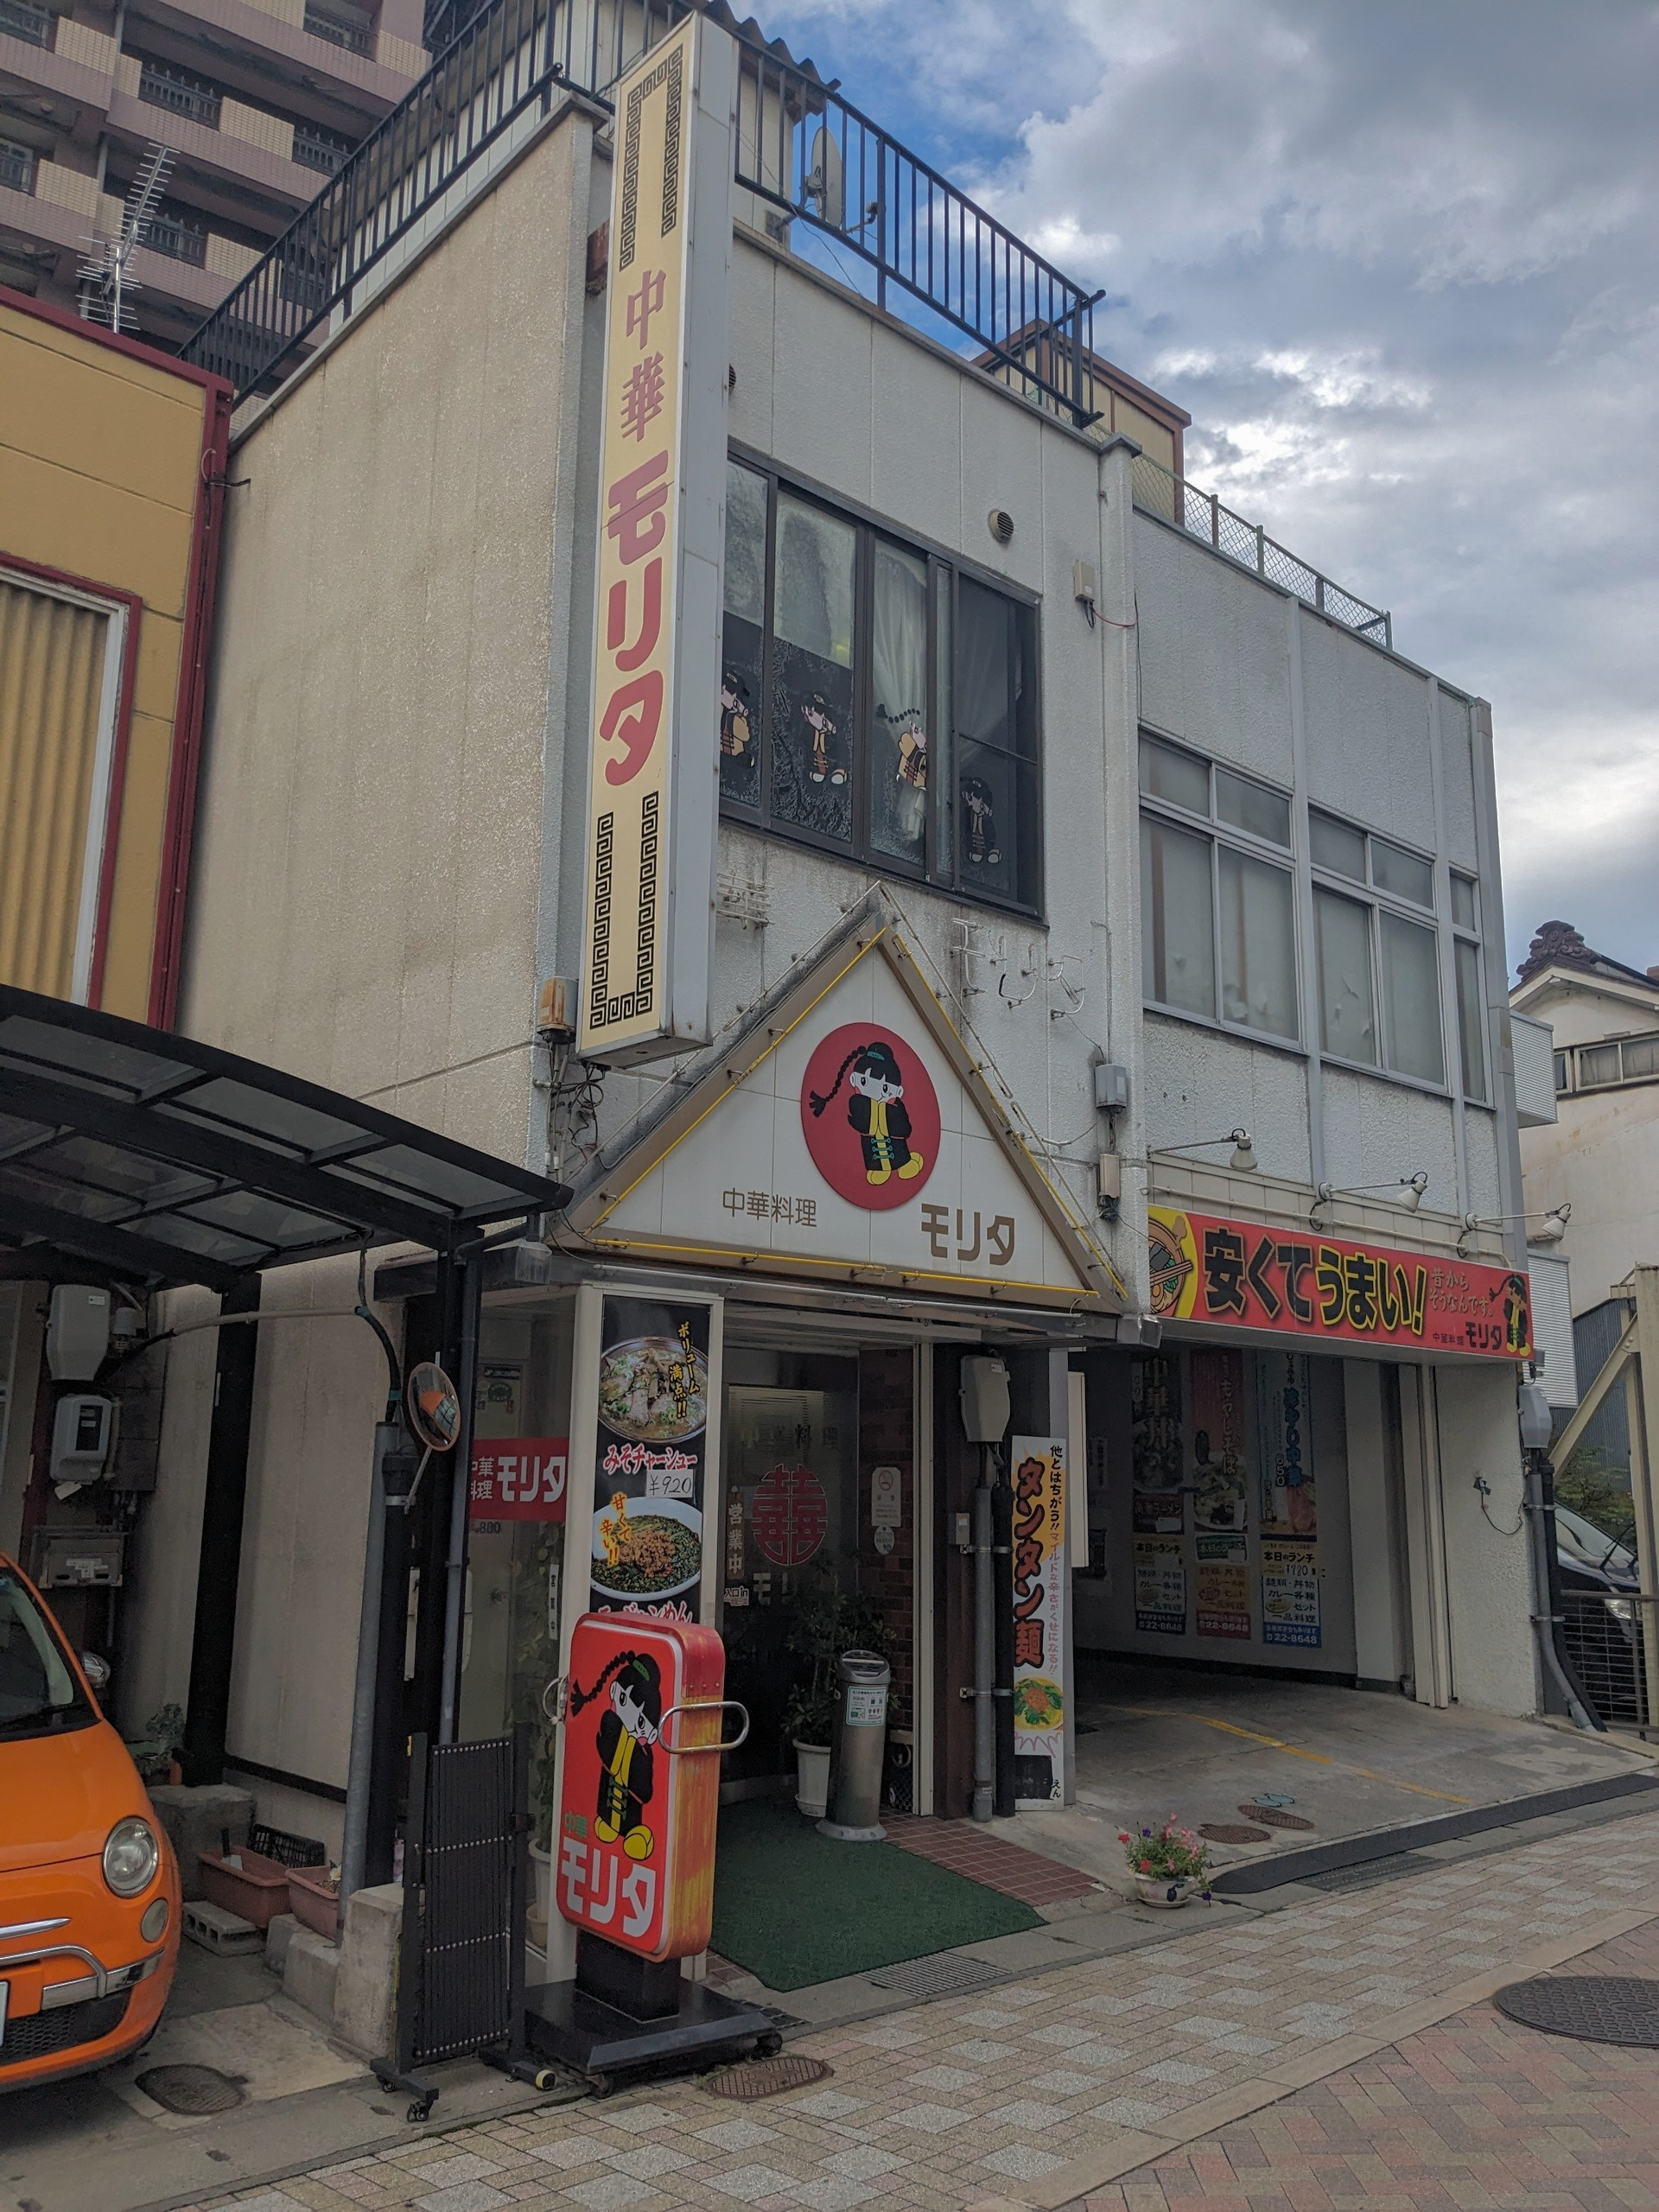
\includegraphics[width=50mm]{c:/Users/user/Documents/ImageProc/task/img/Morita.jpg}
\caption{用意した画像}
\label{Morita}
\end{figure}
図\ref{Morita}のノイズの除去を、周辺画素の中央値を取るメジアンフィルタと、周辺画素の外れ値を除去し平均化するバイラテラルフィルタ
の二種類で行っていく。

本演習で用いたメジアンフィルタとバイラテラルフィルタについて初めに少し説明していく。

メジアンフィルタは上記の通り、周辺画素の中央値をとるフィルタになる。平均値ではなく中央値を取ることで被写体と背景の
境界など輝度や色が大きく変わる場所で、出力の値が大きく外れた値になりづらくなる。このため画像のエッジを保存したまま
平滑化出来るフィルターとなる。

バイラテラルフィルタは、周辺画素の中で輝度値や色が大きく外れている値を除去するレンジフィルタと、周辺画素の平均値を
求める空間フィルタであるガウシアンフィルタの二つをこの順番でかけるフィルタになる。
初めにレンジフィルタで外れ値を除去してから平均値を求めることで、こちらも画像のエッジを保存したまま平滑化できるフィルタである。

\section{処理結果-考察}
以下にガウシアンノイズとソルト\&ペッパーノイズを付加した図\ref{Morita}の画像を図\ref{noise}に示す。
\begin{figure}[h]
    \centering
    \begin{tabular}{cc}
        \begin{minipage}[c]{0.45\hsize}
            \centering
            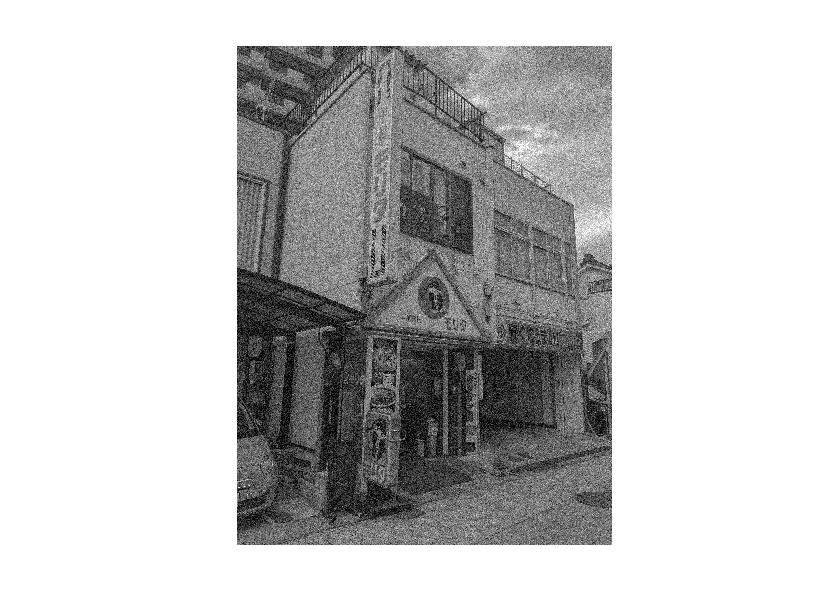
\includegraphics[width=70mm]{./img/gauss_before.jpg}
        \end{minipage}&
        \begin{minipage}[c]{0.45\hsize}
            \centering
            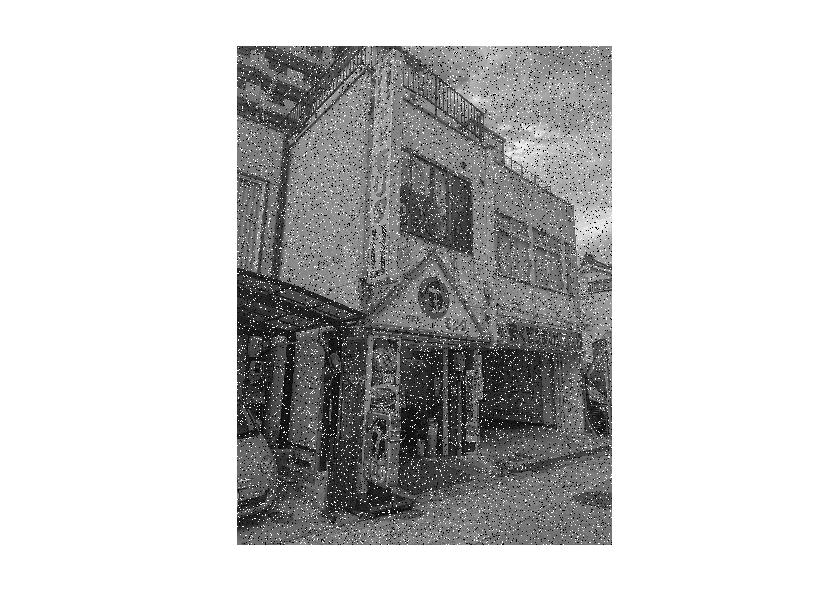
\includegraphics[width=70mm]{./img/sp_before.jpg}
        \end{minipage}
    \end{tabular}
    \caption{ガウシアンノイズ(左図)とソルト\&ペッパーノイズ(右図)を付加した図\ref{Morita}}
    \label{noise}
\end{figure}

図\ref{noise}のようにガウシアンノイズはノイズの輝度値の分布がガウス分布に従ったノイズであり、ソルト\&ペッパーノイズは
白ないしは黒の極端なノイズになる。

この画像をフィルタで処理した結果を以下に示していく。

\subsection{ガウシアンノイズ}
以下ではガウシアンノイズを付加した画像のフィルタリング結果を示していく。

\subsubsection{メジアンフィルタ}
ガウシアンノイズをメジアンフィルタで処理した結果以下の画像\ref{gauss_med}が得られた。
\begin{figure}[h]
    \centering
    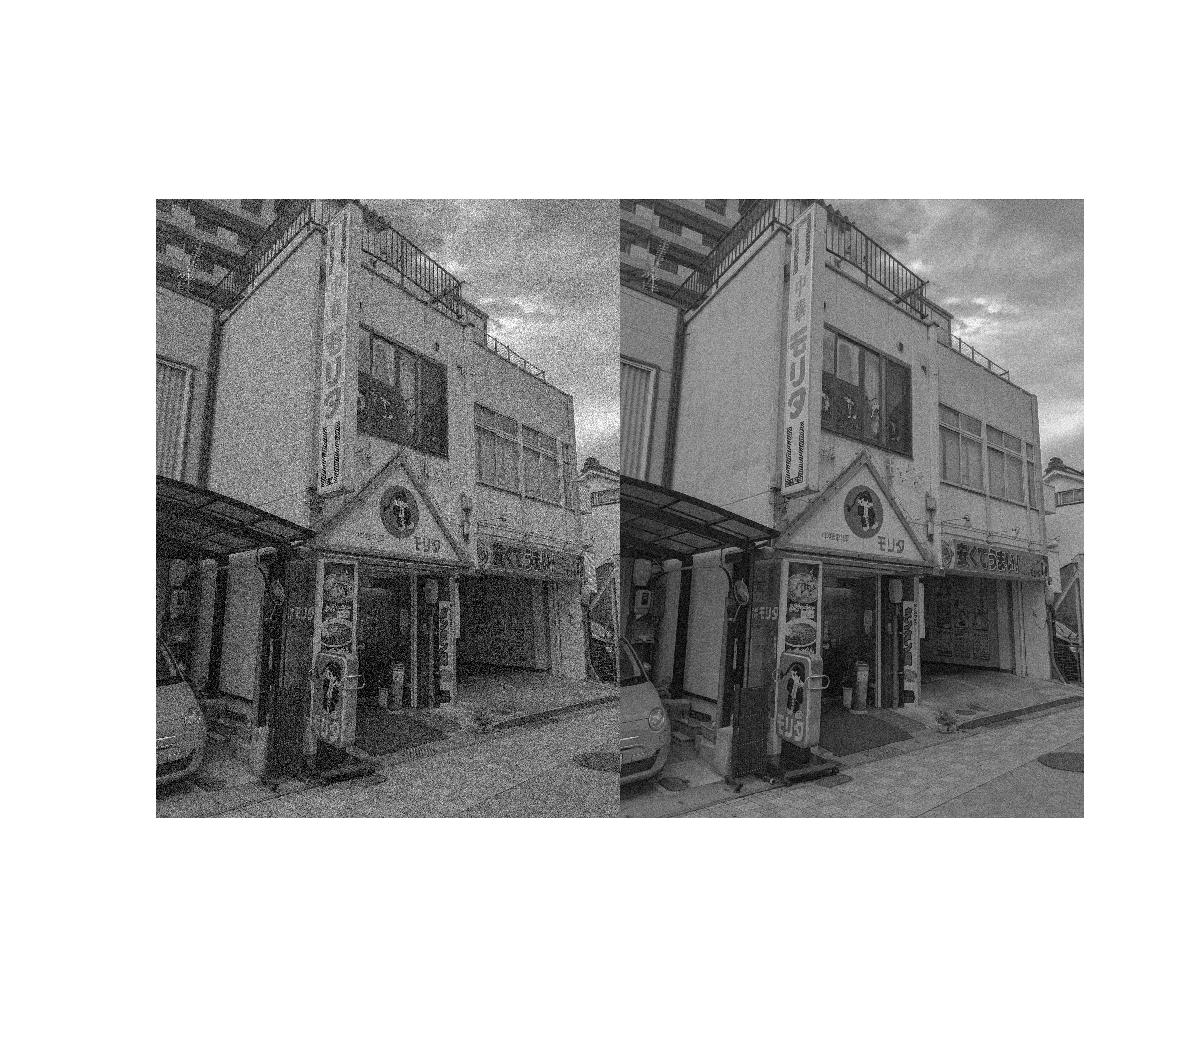
\includegraphics[width=90mm]{./img/gauss_med.jpg}
    \caption{メジアンフィルタでのガウシアンノイズの処理結果}
    \label{gauss_med}
\end{figure}
右の図が処理後の画像となり、少し小さく見えずらいがかなりノイズが取り除けており、鮮明な画像になっていることが分かる。
特に画像中の文字が処理前に比べ視認しやすくなっており、ぷつぷつとしたノイズが取り除けていることが分かる。

\subsubsection{バイラテラルフィルタ}
次にガウシアンノイズをバイラテラルフィルタで処理した結果以下の画像図\ref{gauss_bil}が得られた。
\begin{figure}[h]
    \centering
    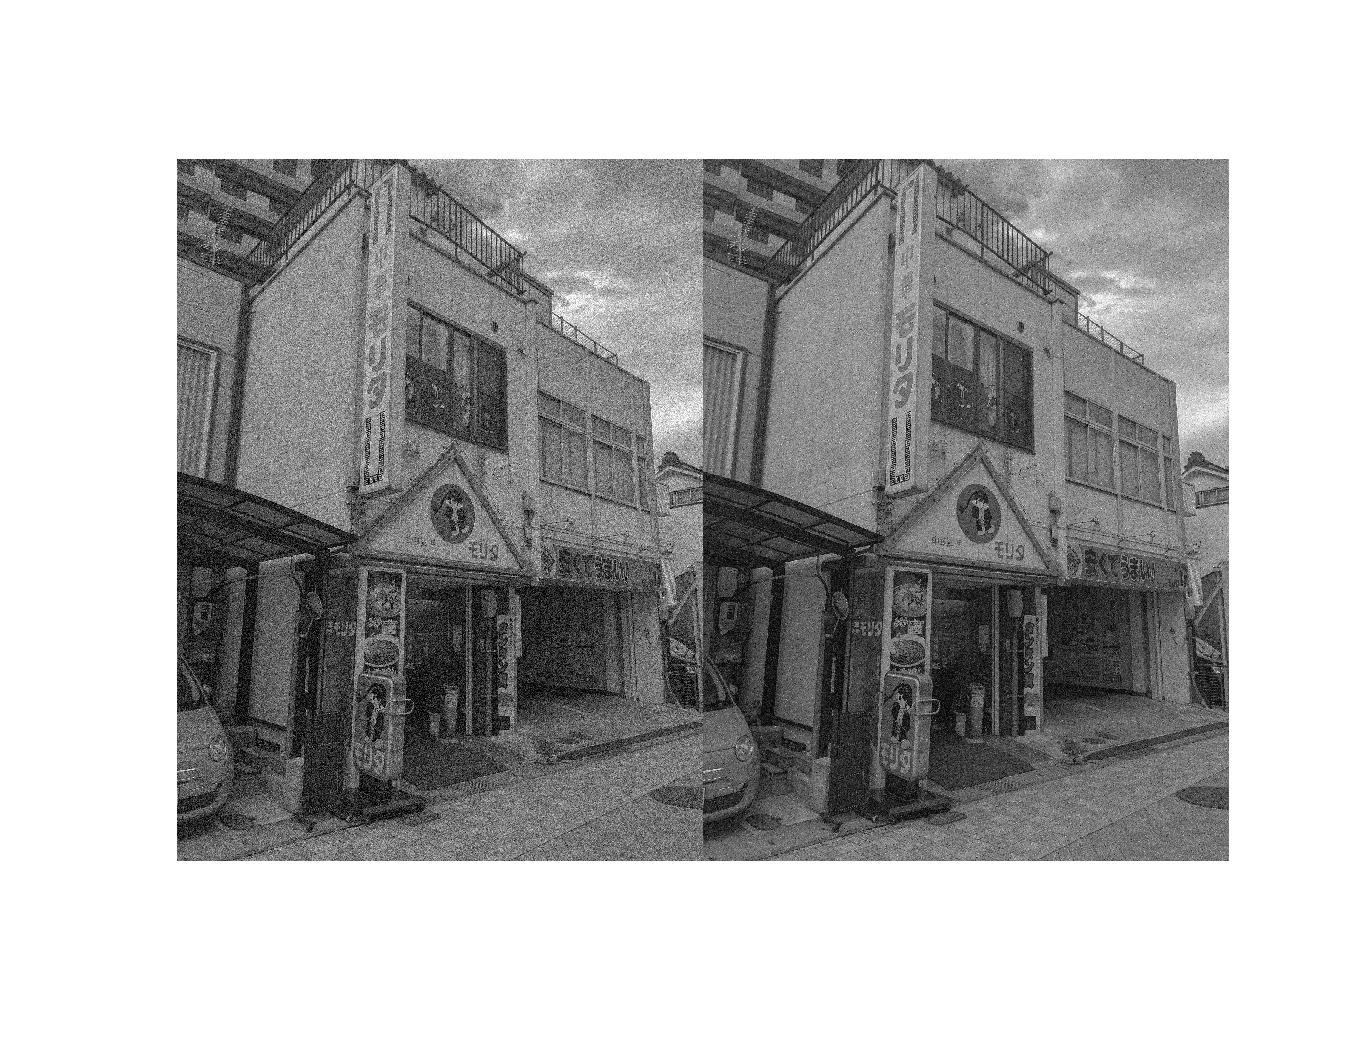
\includegraphics[width=90mm]{./img/gauss_bil.jpg}
    \caption{バイラテラルフィルタでのガウシアンノイズの処理結果}
    \label{gauss_bil}
\end{figure}
こちらも右の図が処理後の画像となる。処理後の画像は背景の空を見ると明確にノイズが取り除けていることが分かるが、
前者のメジアンフィルタよりはあまり鮮明なノイズ除去が出来ておらず、正面入口の"モリタ"の文字もあまり復元できていない。

以上より、ガウシアンノイズによる劣化した画像はメジアンフィルタでの平滑化が適していると考えられる。
実際に処理内容で考察してみると、白と黒の中間の灰色のノイズが多いガウシアンノイズでは、おそらく外れ値と呼べるようなノイズが出てこず、
レンジフィルタでの平滑化がうまく進まなかったのだと考えられる。この点がバイラテラルフィルタの弱点になっていることが分かる。

\subsection{ソルト\&ペッパーノイズ}
続いて以下でソルト\&ペッパーノイズを付加した画像のフィルタリング結果を示していく。

\subsubsection{メジアンフィルタ}
ソルト\&ペッパーノイズをメジアンフィルタで処理した結果以下の画像\ref{sp_med}が得られた。
\begin{figure}[h]
    \centering
    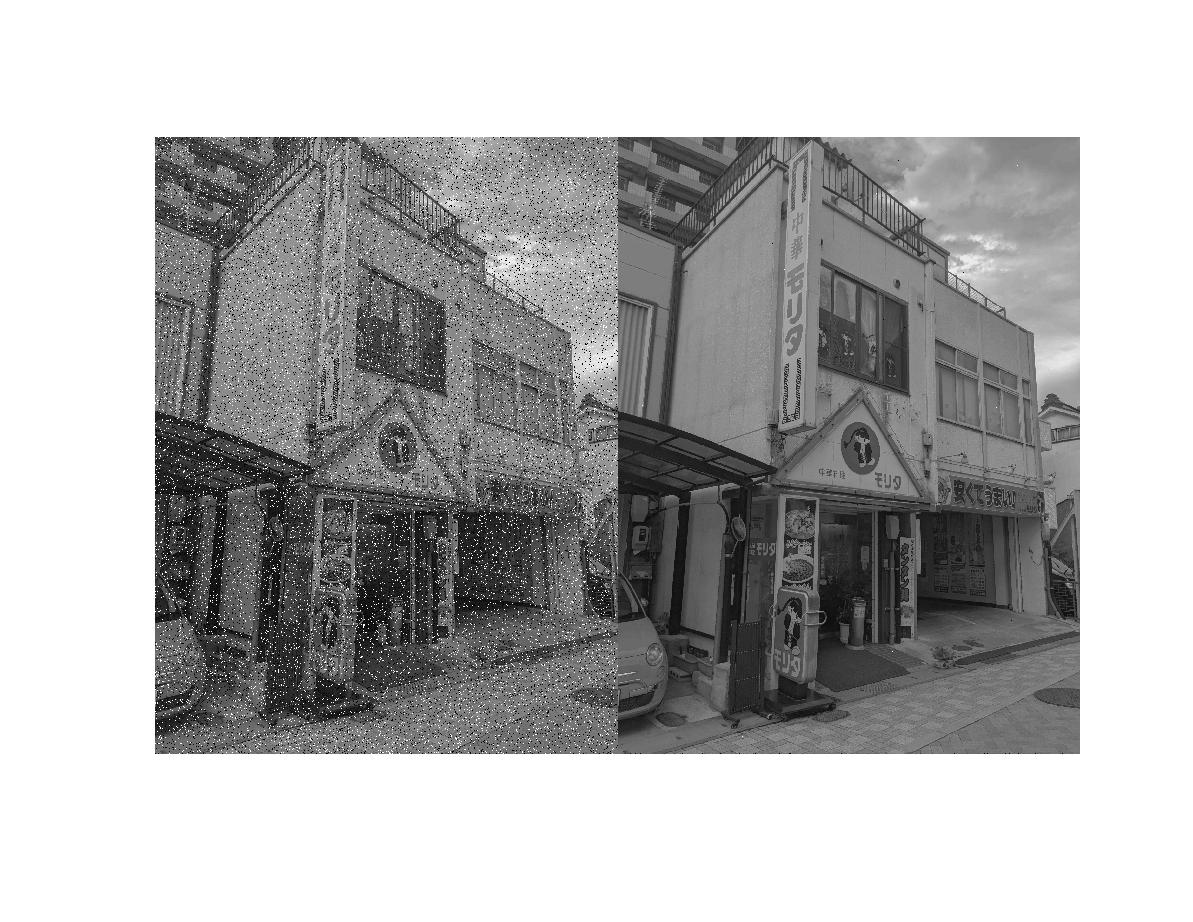
\includegraphics[width=90mm]{./img/sp_med.jpg}
    \caption{メジアンフィルタでのソルト\&ペッパーノイズの処理結果}
    \label{sp_med}
\end{figure}
右の図が処理後の画像となり、少し小さく見えずらいがかなりノイズが取り除けており、鮮明な画像になっていることが分かる。
大きく目立つノイズはなくなっており、元の画像の質感を取り戻しつつ、エッジを保存したままの平滑化が出来ている。

\subsubsection{バイラテラルフィルタ}
次にソルト\&ペッパーノイズをバイラテラルフィルタで処理した結果以下の画像図\ref{sp_bil}が得られた。
\begin{figure}[h]
    \centering
    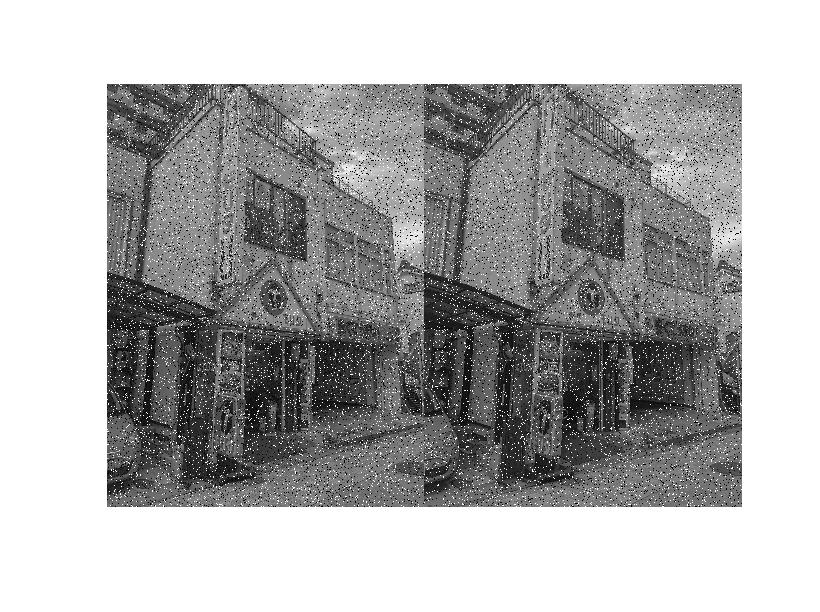
\includegraphics[width=90mm]{./img/sp_bil.jpg}
    \caption{バイラテラルフィルタでのソルト\&ペッパーノイズの処理結果}
    \label{sp_bil}
\end{figure}
こちらも右の図が処理後の画像となる。この図では処理前処理後の画像を比較しても分かるような変化がなく、全くノイズが取り除けていないように見える。
実際にノイズが取り除けているのかどうかこの2画像の差を取った画像を図\ref{sa}に示す。
\begin{figure}[h]
    \centering
    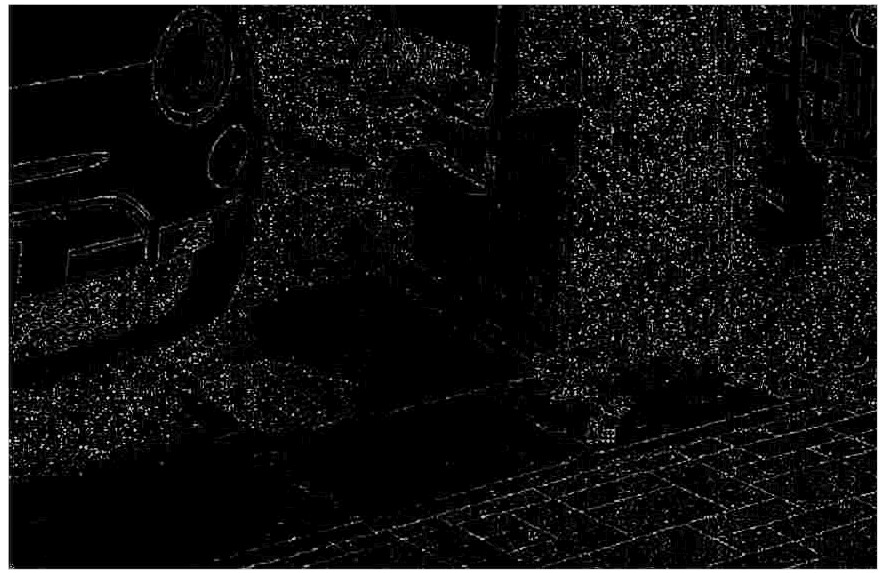
\includegraphics[width=60mm]{./img/untitled~2.jpg}
    \caption{図\ref{sp_bil}の左右の画像差分}
    \label{sa}
\end{figure}

可視性を上げるため、ある程度差を見やすくし、図\ref{Morita}の左下にある車部分を大きく拡大している。
これを見ると確かに処理が施されておりノイズが除去されていることが分かるが、ただ肉眼で見ると全く変化がないように見え、
平滑化ができたとは言えない結果になってしまった。

以上の結果よりソルト\&ペッパーノイズにより劣化した画像の平滑化もメジアンフィルタが適していることが考えられる。

私の演習前の予想としては白黒のノイズが外れ値となり、バイラテラルフィルタをかけたときのレンジフィルタにより除外される
と思っていたがあまりうまく動かなかった。演習に用いたコードに誤りがあったり、適切ではない窓半径を用いてしまったことも
考えられるが、私の力ではここまでの結果しか得られなかった。

最後にこの実験にて用いたコードと条件を示す。ガウシアンフィルタの標準偏差は1、メジアンフィルタの窓サイズは1で行った。
\lstinputlisting[caption={filtering.m}]{c:/Users/user/Documents/ImageProc/task/filtering.m}


\end{document}